\documentclass[aspectratio=169,10pt]{beamer}
\usetheme{default}
\usecolortheme{seahorse}
\setbeamertemplate{navigation symbols}{}
\setbeamertemplate{footline}[frame number]
\usepackage{graphicx, booktabs}
\graphicspath{{../figures/}}

\title{Run\_55 Micro-TPC 3-D Tracking:\\
       Source Pointing, Alignment \& Drift Calibration}
\subtitle{n\_TOF EAR2 X17 --- DREAM Micromegas, scint-doubles trigger,
          $^3$He target (July 18--19, 2026)}
\author{Dylan Neff \\[0.5ex] {\small analysis and slides prepared with Claude
        (Anthropic AI assistant)}}
\date{July 20, 2026}

\begin{document}

\begin{frame}\titlepage\end{frame}

% ---------------------------------------------------------------- overview
\begin{frame}{Where we stand --- one slide}
\begin{itemize}
\item From the 24 recovered run\_55 subruns (76\,214 triggers) a stringent
      realism gate yields \textbf{762 clean X/Y 3-D micro-TPC segments}
      (A 308, B 153, C 287, D 14).
\item The tracks are \textbf{real} (bench charge-balance value, tight vs the
      shuffled null) and they \textbf{point back at the $^3$He source} in all
      eight planes.
\item An \textbf{in-situ source-hypothesis calibration} is in hand per plane:
      transverse alignment ($u_0$), angle scale (charge sharing), and a
      fringe-field distortion map. Drift velocity confirmed on chamber C.
\item \alert{Caveat:} the calibration is fit \emph{assuming} the tracks come
      from the source --- it shows self-consistency, not an independent
      validation. Absolute angle scale / $v_\mathrm{drift}$ stay partly
      degenerate; single-track pointing is resolution-limited ($\sim$11$^\circ$).
\end{itemize}
\vspace{0.5ex}
\footnotesize Data local at \texttt{\~{}/x17/beam\_july/runs/run\_55/}
(combined hits + decoded waveforms). Scripts \texttt{27*} in
\texttt{mx\_july\_beam\_qa/}; full writeup
\texttt{TRACKING\_RUN55\_ANALYSIS.md}.
\end{frame}

% ---------------------------------------------------------------- the picture
\begin{frame}{The micro-TPC picture and the realism gate}
\begin{columns}
\column{.54\textwidth}
\begin{itemize}
\item Each chamber is a single micro-TPC 30 mm from the target; electrons drift
      the gap along the radial normal, strips read $(u,v)=$ (transverse,
      beam-axis).
\item A source track $\Rightarrow$ a \textbf{monotonic full-gap trail}: strip
      position vs peak drift-sample is an ordered line spanning the gap.
\item Gate (per plane): compact ($\leq$25 mm), full-gap peak-time span
      ($\geq$6 samp), trail monotonicity $|\rho|\geq0.8$; then X/Y consistency
      in drift-time, length and charge balance.
\item \textbf{Key discriminator:} use the peak-time span (\texttt{dur}), NOT the
      pulse-envelope --- high-gain single pulses fake full-gap otherwise.
\end{itemize}
\column{.44\textwidth}
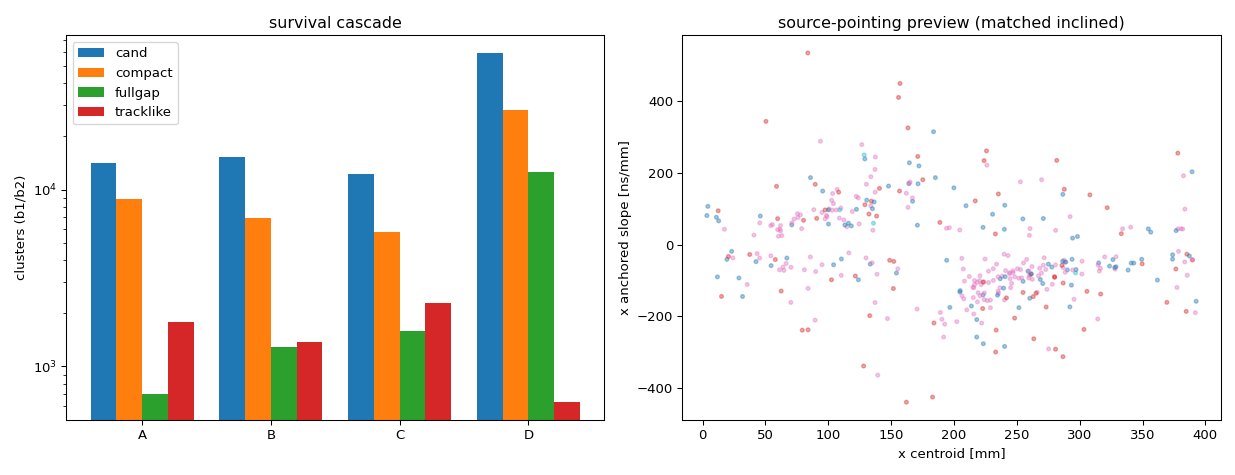
\includegraphics[width=\textwidth]{27_tracks/03_cascade.png}
\footnotesize The survival cascade: D's 59k capture-flood candidates collapse to
354 inclined --- the gate does the contamination rejection it was built for.
\end{columns}
\end{frame}

% ---------------------------------------------------------------- real
\begin{frame}{The tracks are real: charge balance vs the shuffled null}
\begin{columns}
\column{.56\textwidth}
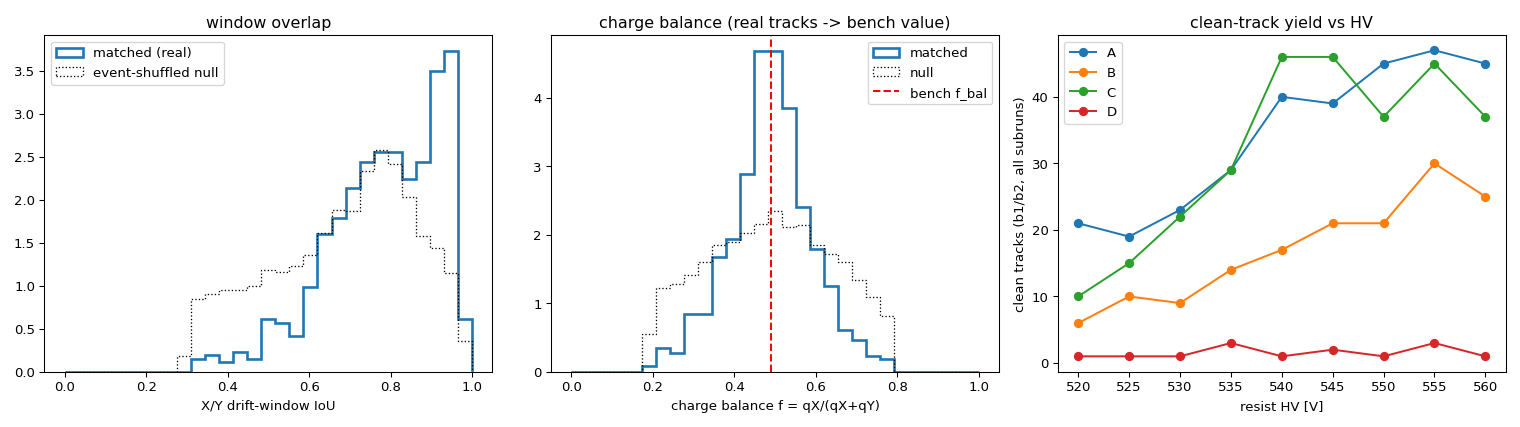
\includegraphics[width=\textwidth]{27_tracks/02_validation.png}
\column{.42\textwidth}
\begin{itemize}
\item Matched X/Y pairs sit at the June \textbf{bench charge-balance}
      $f=q_X/(q_X{+}q_Y)\approx0.48$--$0.50$ and are much \textbf{tighter} than
      the event-shuffled accidental null.
\item Random combinatorics cannot reproduce the bench value at that width
      $\Rightarrow$ the segments are genuine.
\item Track-like multiplicity $\approx$1.04 per plane: 90\% of two-plane events
      are a unique 1$\times$1 pairing.
\item Clean-track yield rises with resist HV for A/B/C (gain turn-on), flat/low
      for D --- same story as the 25b efficiency proxy, now on verified tracks.
\end{itemize}
\end{columns}
\end{frame}

% ---------------------------------------------------------------- calibration
\begin{frame}{In-situ calibration: alignment, angle scale, distortion}
\begin{columns}
\column{.56\textwidth}
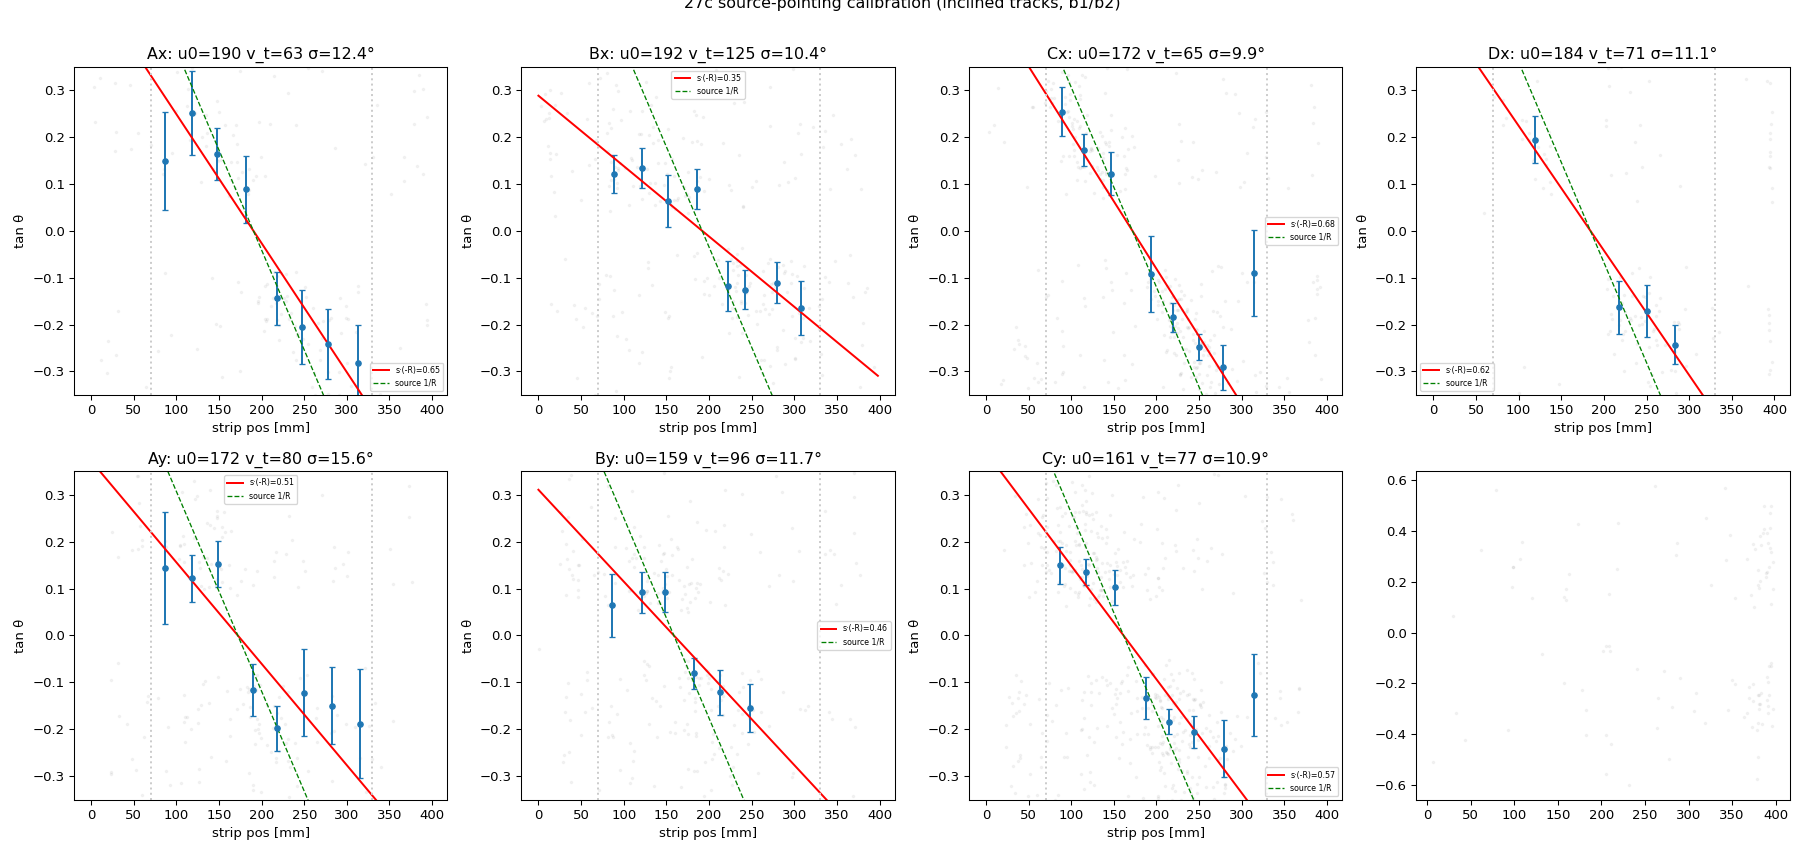
\includegraphics[width=\textwidth]{27_tracks/04_align.png}
\column{.42\textwidth}
\footnotesize
Source model per plane: $\tan\theta = (u-u_0)/R$, $R\approx234$ mm.
Fit $\tan\theta_\mathrm{meas}$ vs $u$ in a 70--330 mm fiducial:
\begin{itemize}
\item \textbf{Alignment} $u_0$: transverse (x) good to \textbf{$\sim$1 cm}
      on all chambers.
\item \textbf{Angle scale} $s\cdot(-R)\approx\mathbf{0.62}$, consistent A/C/D
      --- the $\sim$40\% charge-sharing \emph{compression} of the raw
      time-fit (same bias the bench regression removes), NOT a $v_\mathrm{drift}$
      error. B is the outlier (0.35; wide-cluster/ringing pathology).
\item \textbf{Edge distortion} (next slide): residual flat in-fiducial, turns up
      $\sim$+10$^\circ$ beyond 330 mm in \emph{every} plane $\Rightarrow$ a real
      drift fringe field, mapped in \texttt{calib/27\_align.json}.
\end{itemize}
Stored: \texttt{27\_align.json} ($u_0$, \texttt{scale\_sR},
\texttt{dist\_pos/dtan}, $v_\mathrm{nom}$).
\end{columns}
\end{frame}

% ---------------------------------------------------------------- geometry / pointing (HERO)
\begin{frame}{Realistic geometry \& source pointing}
\includegraphics[width=\textwidth]{27_tracks/14_pointing_geometry.png}
\vspace{-0.5ex}
\footnotesize
\textbf{(a)} Pinwheel of the 4 chambers (A top / C bottom / B left / D right),
beam vertical; calibrated rays fan back onto the $^3$He capsule.
\textbf{(b)} Side view: rays converge \emph{below} centre.
\textbf{(c)} 332 matched segments; reconstructed origin median
\textbf{$(-27,-34)$ mm} vs the $\varnothing20\times40$ capsule. Convergence is
statistical --- single-track pointing $\sim$11$^\circ$.
\end{frame}

% ---------------------------------------------------------------- before/after
\begin{frame}{Before / after calibration on the beam axis}
\begin{columns}
\column{.62\textwidth}
\includegraphics[width=\textwidth]{27_tracks/15_beamaxis_convergence.png}
\column{.36\textwidth}
\footnotesize
\begin{itemize}
\item \textbf{(a)} Raw pointing miss slopes $-110\to+90$ mm across the strip
      (angle-scale undershoot $+$ edge bending); calibrated is \textbf{flat on
      zero} through the fiducial.
\item \textbf{(b)} Beam-axis crossing centroid moves
      \textbf{$-32\to0$ mm} --- onto the source.
\item \alert{Honest read:} calibration removes \emph{bias} and
      \emph{position-dependent distortion}. It does \emph{not} shrink the width
      ($\sigma$ 111$\to$153 mm): single-track pointing is set by the
      $\sim$11$^\circ$ resolution (extended source $\sim$5$^\circ$, near-normal
      short lever, coherent CM noise).
\item The fit is in-sample, so this is a self-consistency / bias-\&-distortion
      demonstration, not an independent validation.
\end{itemize}
\end{columns}
\end{frame}

% ---------------------------------------------------------------- physics: low source + vdrift
\begin{frame}{Two physics results fall out}
\begin{columns}
\column{.46\textwidth}
\textbf{1. The source is $\sim$3 cm low in beam-Y.}
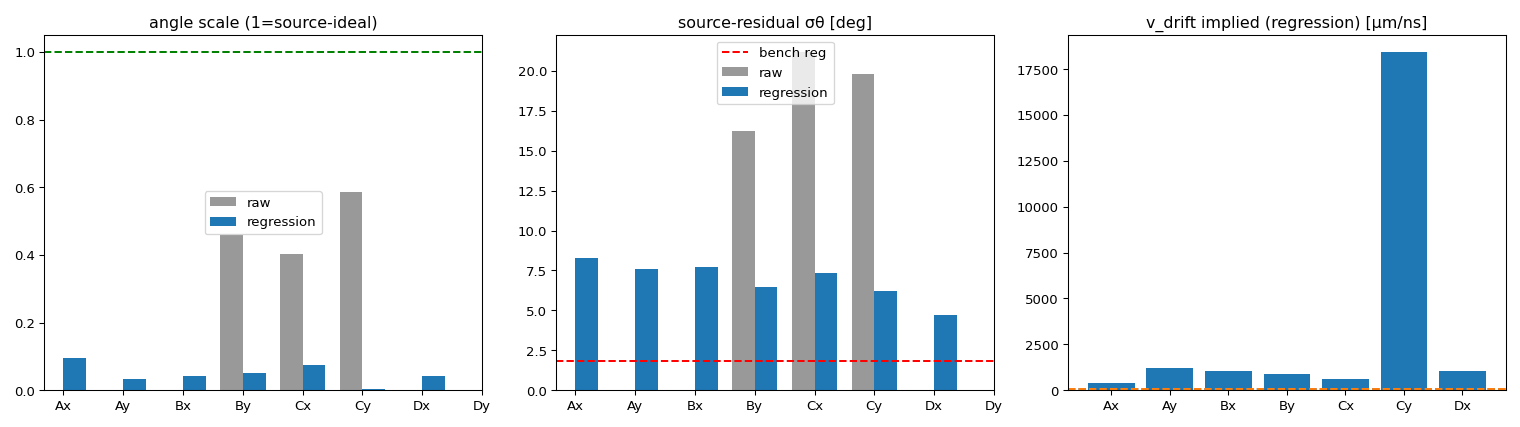
\includegraphics[width=\textwidth]{27_tracks/10_source_loc.png}
\footnotesize
Chambers independently triangulate the same offset (A $-21$, B $-29$, C $-48$
mm). At EAR2 the beam is vertical and neutrons enter the capsule from below, so
captures pile up at the \textbf{bottom} of the $D20\times L40$ capsule --- this
is real source position, NOT a $y$-misalignment to correct.
\column{.50\textwidth}
\textbf{2. Drift velocity, telescope-free.}
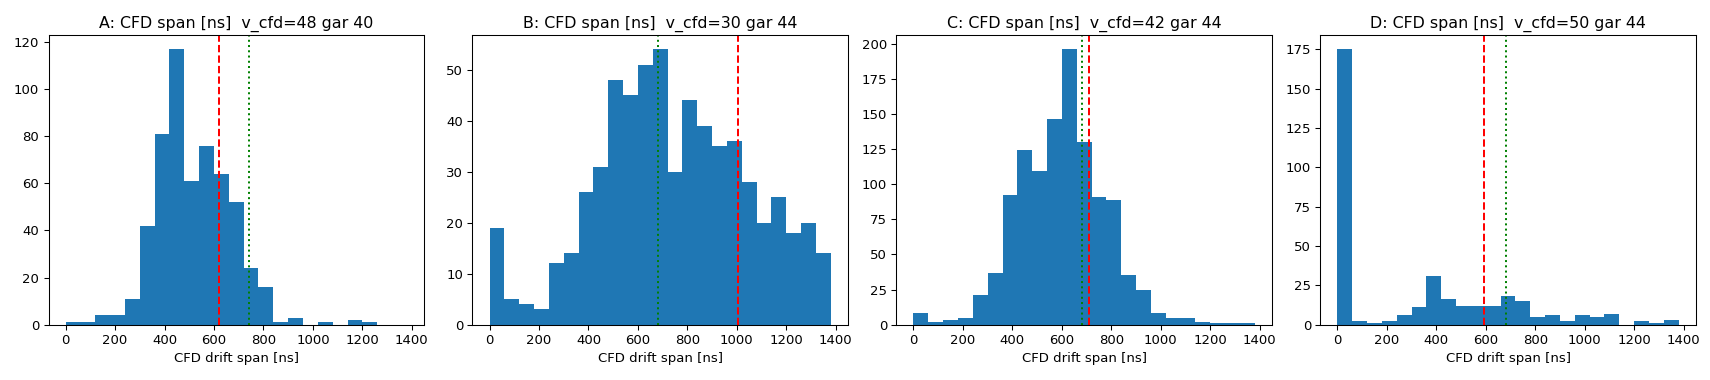
\includegraphics[width=\textwidth]{27_tracks/12_wf_vdrift.png}
\footnotesize
Full-gap drift-time span $=$ gap$/v$, angle-independent. From CFD waveform
reconstruction (2701 tracks): \textbf{C sits on garfield} (42 vs 44 $\mu$m/ns);
A/D read $\sim$10\% high, B low (untrusted). $\Rightarrow$
$v_\mathrm{drift}\approx44$ $\mu$m/ns is consistent for the trusted chamber; the
$\sim$0.6 angle scale is charge sharing, not $v$.
\end{columns}
\end{frame}

% ---------------------------------------------------------------- negative result
\begin{frame}{What does NOT work (yet), and why}
\begin{itemize}
\item \textbf{The frozen bench angle-regressor does not transfer.} Restandardized
      onto run\_55 features, the bench $|\tan|$ model (holdout $\sigma$
      1.7--1.8$^\circ$ on cosmics) collapses --- source-pointing slope $\to0$.
      Cause: it was trained on cosmics spanning a broad angle range; run\_55
      source tracks are \textbf{near-normal incidence} (small, narrow $\tan$), so
      restandardization mis-maps the feature scale.
\item \textbf{Sub-sample timing does not help.} CFD reconstruction of all 2701
      inclined tracks gives the \emph{same} $\sim$0.6 compression and the
      \emph{same} $\sim$11$^\circ$ resolution as the 60 ns max-sample fit
      $\Rightarrow$ the compression is genuine charge sharing and the resolution
      is S/N-limited (coherent CM noise on low-amplitude trail strips), not
      timing-quantisation-limited.
\item \textbf{Everything is b1/b2 windows only} (8--12, 16--28 ms); the 2--6 ms
      physics target is unsampled (the DAQ FIFO comb).
\end{itemize}
\end{frame}

% ---------------------------------------------------------------- calibrated?
\begin{frame}{Are we calibrated?}
\textbf{First-order yes} --- and here is exactly what that means:
\begin{itemize}
\item[\checkmark] \textbf{Alignment}: transverse $u_0$ to $\sim$1 cm, all chambers.
\item[\checkmark] \textbf{Angle scale}: 0.62 charge-sharing compression measured
      and consistent A/C/D.
\item[\checkmark] \textbf{Distortion}: edge fringe-field map per plane; fiducial
      is clean.
\item[\checkmark] \textbf{Drift velocity}: garfield confirmed on chamber C.
\item[\checkmark] \textbf{Pointing}: unbiased; centroid nails the source
      including the $-3$ cm beam-Y physics.
\end{itemize}
\alert{But not closed:}
\begin{itemize}
\item[$\triangleright$] The calibration is \textbf{in-sample} (source-assumed)
      --- self-consistent, not independently validated.
\item[$\triangleright$] Absolute angle scale $\leftrightarrow v_\mathrm{drift}$
      remain \textbf{partly degenerate} (frozen transfer failed).
\item[$\triangleright$] Single-track resolution stuck at $\sim$11$^\circ$
      ($\sim$8--15 cm at the target).
\item[$\triangleright$] B chamber not trusted for scale or $v$.
\end{itemize}
\end{frame}

% ---------------------------------------------------------------- next
\begin{frame}{Follow-ups (in priority)}
\begin{enumerate}
\item \textbf{Re-train the angle regressor in situ} on run\_55 tracks with
      source-truth labels ($\tan\theta=(u-u_0)/R$), holding out for an honest
      residual $\sigma_\theta$ --- this both removes the charge-sharing
      compression and cleanly separates $v_\mathrm{drift}$.
\item \textbf{Improve S/N before precision.} The $\sim$11$^\circ$ resolution is
      coherent-CM-noise-limited on low-amplitude trail strips; reprocess with
      CM correction / ZS ($=1$, 3.5$\sigma$ from the ZS study) to sharpen the
      trail and $v_\mathrm{drift}$.
\item \textbf{Use the low-Y source as the truth anchor} in inter-chamber linking
      / $e^+e^-$ vertexing (ntof\_tracking PLAN\_04); apply the distortion map or
      fiducialize to 70--330 mm.
\item \textbf{Diagnose B} wide-cluster/ringing at the waveform level (also open
      from the HV scan).
\end{enumerate}
\vspace{1ex}
\footnotesize Figures: \texttt{figures/27\_tracks/} (this deck adds
\texttt{14\_pointing\_geometry}, \texttt{15\_beamaxis\_convergence} via
\texttt{27g\_pointing\_geometry.py}). Calibration:
\texttt{calib/27\_align.json}, tracks \texttt{calib/27\_tracks.npz}.
\end{frame}

\end{document}
